% To je predloga za poročila o domačih nalogah pri predmetih, katerih
% nosilec je Tomaž Curk. Avtor predloge je Blaž Zupan.
%
% Seveda lahko tudi dodaš kakšen nov, zanimiv in uporaben element, 
% ki ga v tej predlogi (še) ni. Več o LaTeX-u izveš na
% spletu, na primer na http://tobi.oetiker.ch/lshort/lshort.pdf.
%
% To predlogo lahko spremeniš v PDF dokument s pomočjo programa
% pdflatex, ki je del standardne instalacije LaTeX programov.

\documentclass[a4paper,11pt]{article}
\usepackage{a4wide}
\usepackage{fullpage}
\usepackage[utf8x]{inputenc}
\usepackage[slovene]{babel}
\selectlanguage{slovene}
\usepackage[toc,page]{appendix}
\usepackage[pdftex]{graphicx} % za slike
\usepackage{setspace}
\usepackage{color}
\definecolor{light-gray}{gray}{0.95}
\usepackage{listings} % za vključevanje kode
\usepackage{hyperref}
\renewcommand{\baselinestretch}{1.2} % za boljšo berljivost večji razmak
\renewcommand{\appendixpagename}{Priloge}

\lstset{ % nastavitve za izpis kode, sem lahko tudi kaj dodaš/spremeniš
language=Python,
basicstyle=\footnotesize,
basicstyle=\ttfamily\footnotesize\setstretch{1},
backgroundcolor=\color{light-gray},
}

\title{Celtrin programerski izziv - HTML5 ploščadna igra MyArio}
\author{Primož Pečar }
\date{\today}

\begin{document}

\maketitle

\section{Uvod}

Potrebno je bilo izdelati igro v HTML5 kanvasu, brez zunanjih knjižnjic z uporabo le HTML5, CSS ter javaScript-a. Igra je platformer, navodila niso bila preveč natančna, vendar bilo je rečeno, da se igra obnaša podobno, kot Super Mario ali Sonic, torej platformer, kjer pobiraš kovance se izmikaš nasprotnikom in potuješ po levelu. 

\section{Zamisel}

Igro sem si predstavljal, kot navaden side-scrolling platformer, z različnimi elementi, ki spreminjajo tok igre. Potrebno je bilo izdelati stran, ki je odzivna in prilagodljiva za različne naprave. Predstavljal sem si igranje v položnem načinu telefona, saj imamo tako daljši level, kot v večina platformerjih (naproti navadnem pokončem načinu, kjer imamo ozek in visok level, sicer lahko tudi tako igramo, vendar je uporabnjiška izkušnja slabša).

\section{Izzivi}

V javascriptu sem začel programirati kakšno leto nazaj, izdelal sem že 1 igro, vendar z THREEjs-u, kateri ti poenostavi veliko zadev, ki sem jih moral tukaj narediti iz ničesar, na novo je bilo tudi programiranje na 2d canvasu, do sedaj sem programiral le v 3D svetu. 

\subsection{Odziven dizajn}

Ker se igra poganja v brskalniku in namenjena je za telefone, je bilo potrebno narediti tako okolje, ki se prilagaja obračanju zaslona, različnim dimenzijam ekranov, različnim DPI-jem. Ko sem igro razvijal, sem uporabljal brskalnik chrome, kateri tudi omogoča izvajanje strani v načinu mobitela, igra tudi deluje na firefox brskalnikih vendar se pojavijo napake (firefox drugače rendera canvas, zato se pojavijo črte pri izrisu). Spletna stran se prilagaja vsem možnim napravam, testiral sem na samsung telefonih (v živo), ter iPhone, iPad (v browserju), na večina napravah igra dela dokaj vredu, problemi se pojavijo pri verzijah brskalnikov, saj nekateri ne resizajo canvasa, zaradi URL toolbara zgoraj in imamo posledično kontrole zamaknjene malo izven zaslona.

\subsection{Tilemapping}

Prvotno sem poskušal vse delati v pikslih, torej izris vsega je bil na canvas po x,y koordinatah. To se izkaže za nočno moro saj je nemogoče preverjati collision detectiona, movement je skoraj nemogoč po nekih fizikalnih pravilih in sem to kmalu zavrgel. 
Odločil sem se za tilemapping, tilemapping ti omogoča, da igralčev pogled na igro razdeliš na tako imenovan tile map. Tile map predstavlja celoten ekran, razdeljen na "blokce". Tako lahko celotno igralno površino predstavimo kot en ogromed 2d seznam, kjer pa imamo vrednosti vsakega blokca posebaj. Tako samo spremenimo parameter v seznamu in posledično tudi karekteristiko igre. Kot primer, v moji igri imam vseskupaj 6 različnih blokcov:
\begin{enumerate}
	\item Block 0 predstavlja backgroud, background ne vpliva na igralca, je pomemben samo za izris
	\item Block 1 predstavlja tile oz. površino v katero se lahko zabijemo, celoten level je sestavljen iz
	različnih sekvenc Blokov 1
	\item Block 2 predstavlja sonce, sonca pobiramo in s tem višamo svoj score
	\item Block 3 predstavlja luno, luna poveča št. platform, ki jih lahko postavlja igralec
	\item Block 4 predstavlja sovražnika, ta se premika po mapi
\end{enumerate}
\pagebreak
\subsection{Detekcija kolizij}

Ker nismo smeli uporabljati nobenih zunanjih knjižnjic, je bilo potrebno razviti svoj fizikalni model. Z tile mappingom se nisem nikoli ukvarjal, kar mi je delalo velike probleme pri detekciji kolizij. Zastopil sem idejo za AABB collision detectionom, vendar, ker tudi sam ne poznam dobro canvas nisem vedel kako ta stvar rendera zadevo, potrebno je blo blokec razdeliti na 4 dele: Top, bottom, left, right. Na podlagi tega pa se potem sprašuješ ali je pozicija igralca v svetu + njegova hitrost enaka takemu blokcu v mapi, da se vanj zabijemo, če je, igralca zamaknemo nazaj (simuliramo kolizijo), sicer pa pustimo, da gre naprej.

\begin{figure}[htbp]
	\begin{center}
		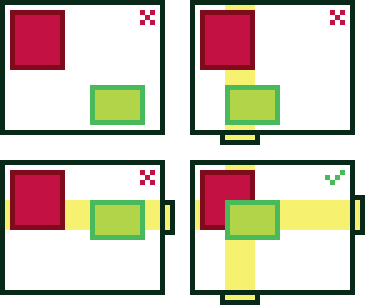
\includegraphics[scale=0.6]{overlap.png}
		\caption{AABB collision detection.}
		\label{zanri_slika}
	\end{center}
\end{figure}
\pagebreak

\subsection{Sidescrolling - Pozicija v svetu}

Sidescrolling je velik del platfomer iger, saj nebi bilo zanimivo, če bi bil lahko samo v enem delu mape. Zato je bilo potrebno implementirati način, da se premikamo po mapi. Sam igralec je omejen na lokalen viewpoint, katerega ne spreminjamo, ta pa je enak dolžina ekrana/velikost bloka * višina ekrana/velikost bloka.

Za simulacijo scrollanje pa je potrebno premikati ta viewpoint. Kar naredim je, da ko se igralec pomika levo/desno in je pri 1/4 koncu ali začetku ekrana začnem premikat celoten svet naprej/nazaj. S tem moramo definirati 2 stvari in to je tileOffsetX in worldOffsetX (v resnici sem imel tudi tileOffsetY in worldOffsetY, vendar sem na koncu zavrgel, ker sem imel veliko več problemov s temi vrednostimi in nisem imel nobene koristi od njih).

Vredno je omeniti, da posledično, ko zamikam igralca in svet se detekcija kolizij ne synca pravilno in lahko pride do napak kot je lebdenje ali pa zatik v bloku. To se reši samo od sebe, ko se collision synca (problem je ker rendaramo -4 +4 bloke naprej nazaj, te pa se ne upoštevajo v collision detectionu in zanjo nastati problemi)

\subsection{Generacija terena}

Teren se generira na podlagi že obstoječega spawn point-a. Kar delamo je dodajamo različne oblike v mapo, da postane bolj dinamična. Tako je svet sestavljen iz platform, floating platfrom, square, wall. Vse imajo naključno velikost in dolžino.

\subsection{Mobilen naičn / PC}

Na podlagi naprave, kjer se igra zažene se igra prilagodi. V primeru, da igramo na telefonu se izrišejo še dodatni HUD elementi, za premikanje. Tudi mapa se prilagaja velikosti naprav, tako da če bo naprava dimenzije 100000000x10000000 se bo pravilo tudi generirala mapa. Tako da podprte so vse možne naprave na tem svetu, vendar zadovoljstvo igralca ni zagotovljeno. V primeru da igramo na računalinku se HUD elemetni pobrišejo, in igro igramo z up,left,right,space.

\subsection{Enemy}

Enemy se tako kot večina stvari v tej igri naključno generira, določeno ima višino, širino in hitrost. Sovražnik se pojavi na vsake 65 blokov, in se počasi premika proti igralcu.

\subsection{Konec igre}

Igra ce ustavi, ko igralec umre 3-krat. Umre tako, da pade v luknjo, ali pa ima kolizijo z sovražnikom. Po koncu igre se izpiše endgame screen in št. točk, ki jih doseže.

\subsection{Player power - spawn tiles}

Med razvojem sem se igral z postavljanjem platformami na različnih nivojih, kar sem ugotovil je to, da lahko to uporabim v načinu igranja, tako lahko igralec pod sabo kreira platformo na kateri stoji, to se izkaže za zelo uporabno po prvih 200 blokcih igre, saj takrat izgine spodni del mape in je igralec prisiljen v težavno platformanje. Število platform je na začetku omejeno na 5, vendar med igranjem lahko pobere luno, katera mu da 2 platforme, ali nekaj 20.

\section{Končna misel}

Sam projekt je bil zanimiv, vendar večkrat med programiranjem sem čutil krutosti javascripta in njegovih errorv. Za nekoga, ki se še nikoli ni ukvarjal s takimi stvarmi je bila to dobra izkušnja za učenje in razumevanje game developmenta. Vendar, nesmiselno se mi je zdelo izumljat tople vode, narediti svoj collision detection in sidescrolling, stvari, ki so že perfektno implementirane v knjižnjicah kot phaser (razen, če Celtro zanima kako dobro posameznik programi HTML5 canvas, drugače pa ne vidim smisla).

\begin{figure}[htbp]
	\begin{center}
		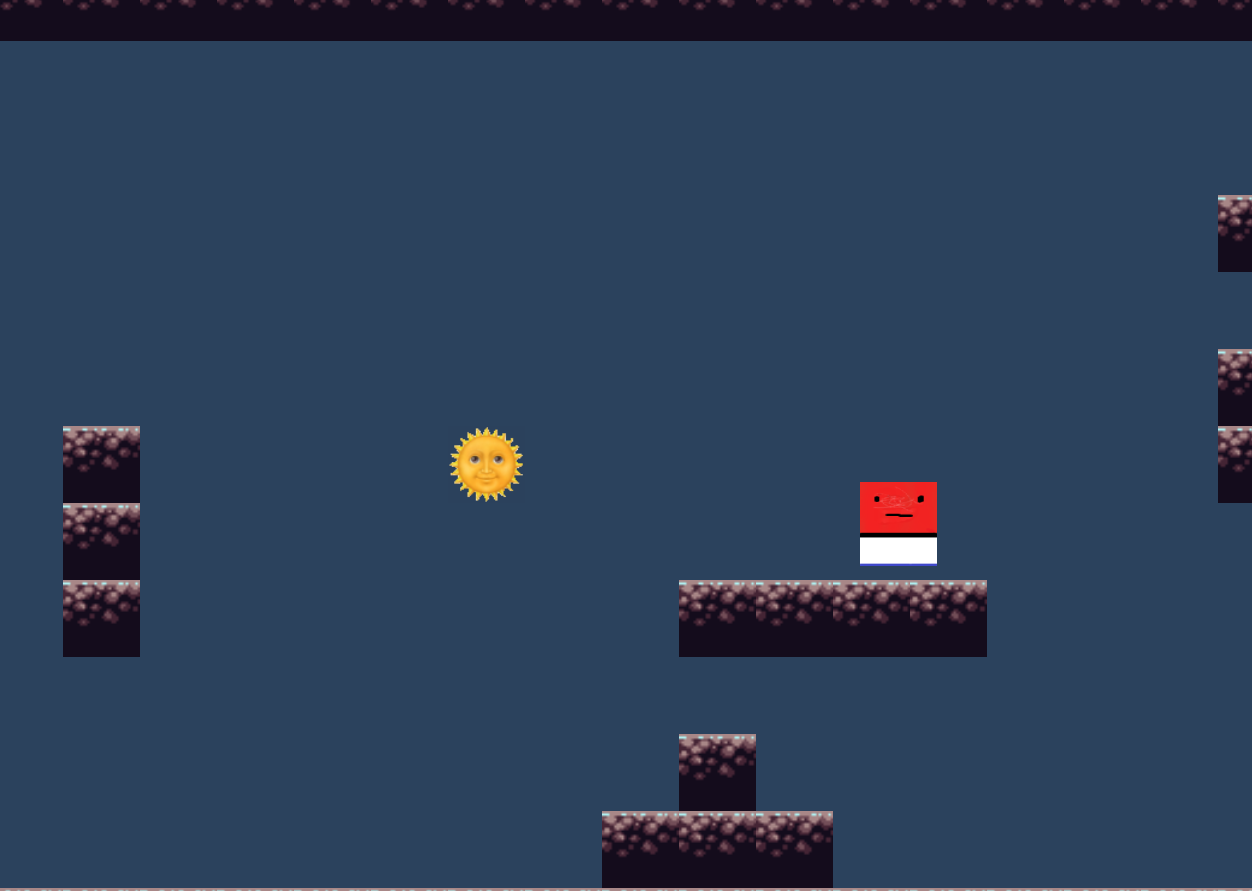
\includegraphics[scale=0.4]{thegame.png}
		\caption{The end.}
		\label{game_scr}
	\end{center}
\end{figure}
\pagebreak

\section{Koda in kontakt}

Koda se nahaja v mapi scripts, če hočete igro zagnati priporočam brskalnik chrome. Če zaganjate preko računalnika:
\begin{enumerate}
	\item Odpri index.html ali \url{http://ppceltra.s3-website.eu-central-1.amazonaws.com/}
	\item Pritistni F12
	\item Namesto responsive device izberi iPhone 5
	\item Zarotiraj telefon z pritiskom gumba na desno in osveži strani
\end{enumerate}

Če zaganjate preko telefona:
\begin{enumerate}
	\item Odpri index.html ali \url{http://ppceltra.s3-website.eu-central-1.amazonaws.com/}
	\item Zarotiraj napravo
	\item Osveži stran
\end{enumerate}

Projekt in pripadajoče programe sem izdelal sam. Kontakt na: pppecar@gmail.com




\end{document}
